\documentclass[11pt]{article}

\usepackage[a4paper, margin=1in]{geometry}
\usepackage{graphicx}
\usepackage{booktabs}
\usepackage{amsmath}
\usepackage{hyperref}
\usepackage{float}
\usepackage{enumitem}
\usepackage{parskip}
\usepackage{microtype}

\hypersetup{
  colorlinks=true,
  linkcolor=blue,
  urlcolor=blue,
  citecolor=blue
}

\title{Detecting Patronising and Condescending Language (PCL) \\
Natural Language Processing Coursework 2026}
\author{Darius Aron \\
Leaderboard Name: \texttt{dodo} \\
GitHub Repository: \url{https://github.com/darius024/pcl-classifier}}
\date{}

\begin{document}

\maketitle
\thispagestyle{empty}

\newpage
\tableofcontents
\newpage

% ============================================================
\section{Introduction}

Patronising and Condescending Language (PCL) is a subtle and socially harmful form of communication that often targets vulnerable communities such as the homeless, disabled, or refugees. Unlike overt hate speech, PCL can be difficult to detect because it is typically embedded within ostensibly positive or neutral framing — for example, describing vulnerable people as helpless or in need of saving, rather than as agents capable of self-determination.

This report describes work carried out for the SemEval 2022 Task 4, Subtask 1 shared task, which frames PCL detection as a \textbf{binary classification problem}: given a news paragraph, classify it as either containing PCL (class~1) or not (class~0). The evaluation metric is the F1 score of the positive (PCL) class, which is appropriate given the strong class imbalance in the dataset.

The report follows the six stages of the NLP research lifecycle as specified in the coursework. Section~\ref{sec:review} presents a critical review of the original PCL dataset paper. Section~\ref{sec:eda} describes two distinct exploratory data analysis techniques applied to the dataset. Section~\ref{sec:approach} proposes and justifies our modelling approach. Section~\ref{sec:global} covers global evaluation and submission confirmation. Section~\ref{sec:local} presents local evaluation including error analysis and a precision--recall study. Sections~\ref{sec:discussion} and~\ref{sec:conclusion} discuss findings and conclude.

% ============================================================
\section{Exercise 1: Critical Paper Review}
\label{sec:review}

\subsection{Q1: Primary Contributions}

The paper ``Don't Patronize Me! An Annotated Dataset with Patronizing and Condescending Language towards Vulnerable Communities'' by Pérez-Almendros et al.\ (2020, updated 2022 for SemEval) makes three primary contributions:

\begin{itemize}
    \item \textbf{Dataset:} The authors introduce the \emph{Don't Patronize Me!} (DPM) corpus, consisting of over 10,000 paragraphs extracted from English-language news articles, each manually annotated for the presence of PCL towards vulnerable communities. Critically, annotations are made at both the document level (binary PCL/No-PCL) and the text-span level — annotators highlight the specific spans that contain PCL — enabling fine-grained supervision at multiple levels. The paragraphs were collected by keyword search (e.g., ``homeless'', ``refugee'', ``disabled'') across articles from many countries, providing broad coverage.

    \item \textbf{Taxonomy:} The paper proposes a two-level, hierarchical taxonomy of PCL types focused on language directed at vulnerable communities. The first level distinguishes PCL from non-PCL. The second level decomposes PCL into seven fine-grained categories: \emph{Unbalanced Power Relations}, \emph{Shallow Solution}, \emph{Presupposition}, \emph{Authority Voice}, \emph{Metaphor}, \emph{Compassion}, and \emph{The Poorer the Merrier}. This taxonomy brings conceptual clarity to a previously informal notion, making annotation reproducible and enabling multi-label classification (Subtask 2 of SemEval 2022).

    \item \textbf{Shared task organisation:} The authors organised SemEval 2022 Task 4, which challenged teams worldwide to build classifiers for binary PCL detection (Subtask 1) and fine-grained PCL category identification (Subtask 2). The shared task provided a standardised benchmark with official train/dev/test splits, evaluation scripts, and a leaderboard, promoting fair comparison across systems.
\end{itemize}

\subsection{Q2: Technical Strengths}

\begin{itemize}
    \item \textbf{Originality and domain novelty:} PCL directed at vulnerable communities had received almost no prior computational treatment. This work fills a clear gap by operationalising a socially important phenomenon that sits between well-studied domains such as hate speech and sarcasm detection. The taxonomy itself is a standalone scholarly contribution that could inform future annotation guidelines and datasets.

    \item \textbf{Annotation rigour:} The authors employed a multi-annotator setup with trained annotators, reported inter-annotator agreement (IAA) using standard metrics (Fleiss's $\kappa$), and used a majority-voting scheme to produce the final binary labels. The annotation guidelines were developed iteratively through calibration rounds, which increases the reliability of gold labels and reduces the risk of systematic annotator bias.

    \item \textbf{Evaluation design:} The choice of F1 score on the positive (PCL) class as the primary metric is well-motivated given the strong class imbalance (roughly 10\% PCL). Accuracy would be misleading — a model that always predicts ``No PCL'' achieves $\sim$90\% accuracy with no useful signal. F1 on the minority class directly captures both precision and recall for the phenomenon of interest.
\end{itemize}

\subsection{Q3: Weaknesses}

\begin{itemize}
    \item \textbf{Low inter-annotator agreement:} The paper reports low IAA scores, attributed to the inherent subjectivity of PCL. While this is acknowledged, the analysis is superficial. There is no investigation into \emph{which} PCL categories or \emph{which} severity levels drive the most disagreement, nor whether specific annotator pairs systematically diverge. A deeper breakdown would clarify whether the low agreement reflects genuine ambiguity in the phenomenon or inconsistencies in the guidelines that could be addressed. More annotators or a different elicitation process (e.g., pairwise comparison rather than independent labelling) might have yielded higher and more stable agreement.

    \item \textbf{Shallow model analysis:} The baseline models presented (including RoBERTa-base) are described without detailed justification for hyperparameter choices such as learning rate, batch size, or class weighting strategy. There are no ablation studies showing the contribution of individual design decisions. Without such analysis, it is hard to tell whether the reported F1 of 0.48 is a reasonable lower bound or whether better tuning of the same architecture could have yielded significantly higher results.

    \item \textbf{Limited generalisation discussion:} The dataset is drawn exclusively from English-language news articles via keyword-based search, meaning all examples are topically anchored to the chosen vulnerable-community terms. The authors do not discuss whether the taxonomy and models would generalise to other domains (e.g., social media, parliamentary speech, or informal text), other languages, or PCL targeting groups not included in the keyword list. The keyword-seeded collection strategy also risks introducing spurious correlations between keywords and labels that could inflate model performance without reflecting genuine PCL understanding.
\end{itemize}

% ============================================================
\section{Exercise 2: Exploratory Data Analysis (EDA)}
\label{sec:eda}

\subsection{EDA Technique 1: Class Distribution and Token Length Analysis}

\subsubsection*{Visual/Tabular Evidence}

\begin{figure}[H]
\centering
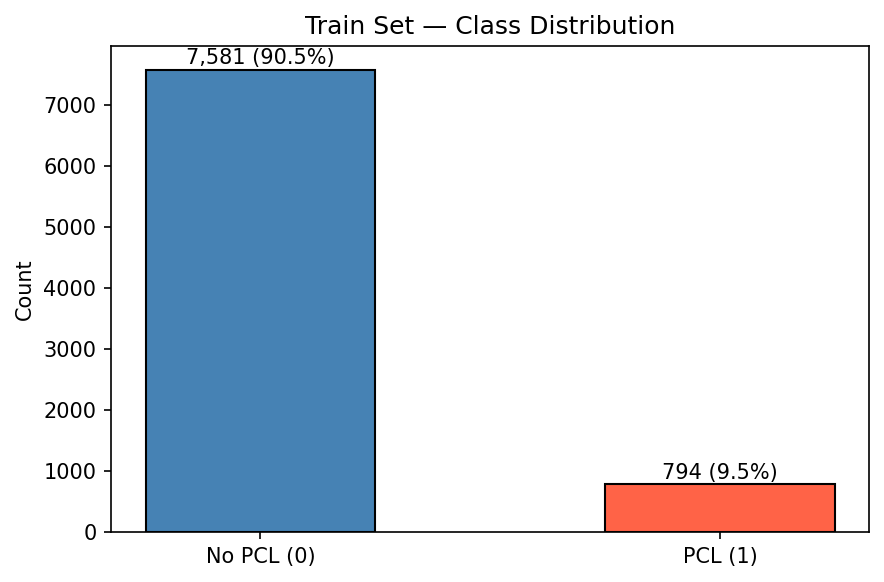
\includegraphics[width=0.62\textwidth]{images/class_distribution.png}
\caption{Class distribution of the full DPM corpus (10,469 examples). The dataset contains 993 PCL examples (9.5\%) and 9,476 No-PCL examples (90.5\%).}
\label{fig:class_dist}
\end{figure}

\begin{figure}[H]
\centering
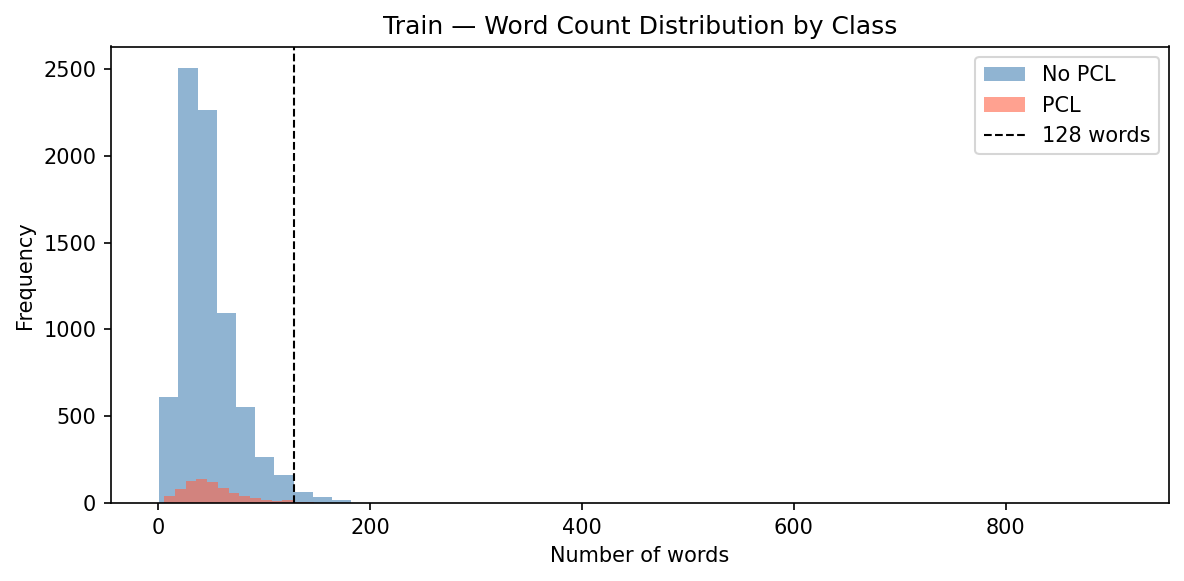
\includegraphics[width=0.7\textwidth]{images/token_lengths.png}
\caption{Token length distribution by class (PCL vs.\ No PCL) in the training set. PCL examples tend to be slightly longer, but both distributions share a similar median.}
\label{fig:token_len}
\end{figure}

\subsubsection*{Analysis}

The DPM corpus contains 10,469 examples in total: 993 PCL (9.5\%) and 9,476 No-PCL (90.5\%), reflecting a roughly \textbf{9.5:1 class imbalance}. This ratio is uniformly preserved across the official train split (8,375 examples; 794 PCL, 9.5\%) and the dev split (2,094 examples; 199 PCL, 9.5\%). The imbalance is severe but not pathological — with $\sim$794 positive training examples there is still meaningful signal for a fine-tuned transformer.

The token length distributions show that PCL examples have a slightly higher mean word count ($\sim$80--100 words) compared to No-PCL examples, though the medians are closer. More importantly, both distributions have a long tail: some examples exceed 300 words, though the 95th percentile is below 200 words.

\subsubsection*{Impact Statement}

The severe class imbalance directly motivates two modelling decisions:

\begin{enumerate}[noitemsep]
    \item \textbf{Weighted Random Sampler (WRS):} During training, examples are sampled proportionally to the inverse of their class frequency. This ensures each mini-batch contains a roughly equal number of PCL and No-PCL examples, preventing the model from learning a trivially high-accuracy solution of always predicting ``No PCL''. Without this, the gradient signal from the minority class would be overwhelmed.
    \item \textbf{\texttt{max\_length=256}:} Setting the transformer input length to 256 tokens captures the 95th percentile of sequence lengths without truncating most examples, while remaining computationally feasible. Sequences above this threshold are truncated, which affects fewer than 5\% of examples.
\end{enumerate}

\newpage

\subsection{EDA Technique 2: Lexical Analysis --- Log-Odds Contrast and Distinctive N-grams}

\subsubsection*{Visual/Tabular Evidence}

\begin{figure}[H]
\centering
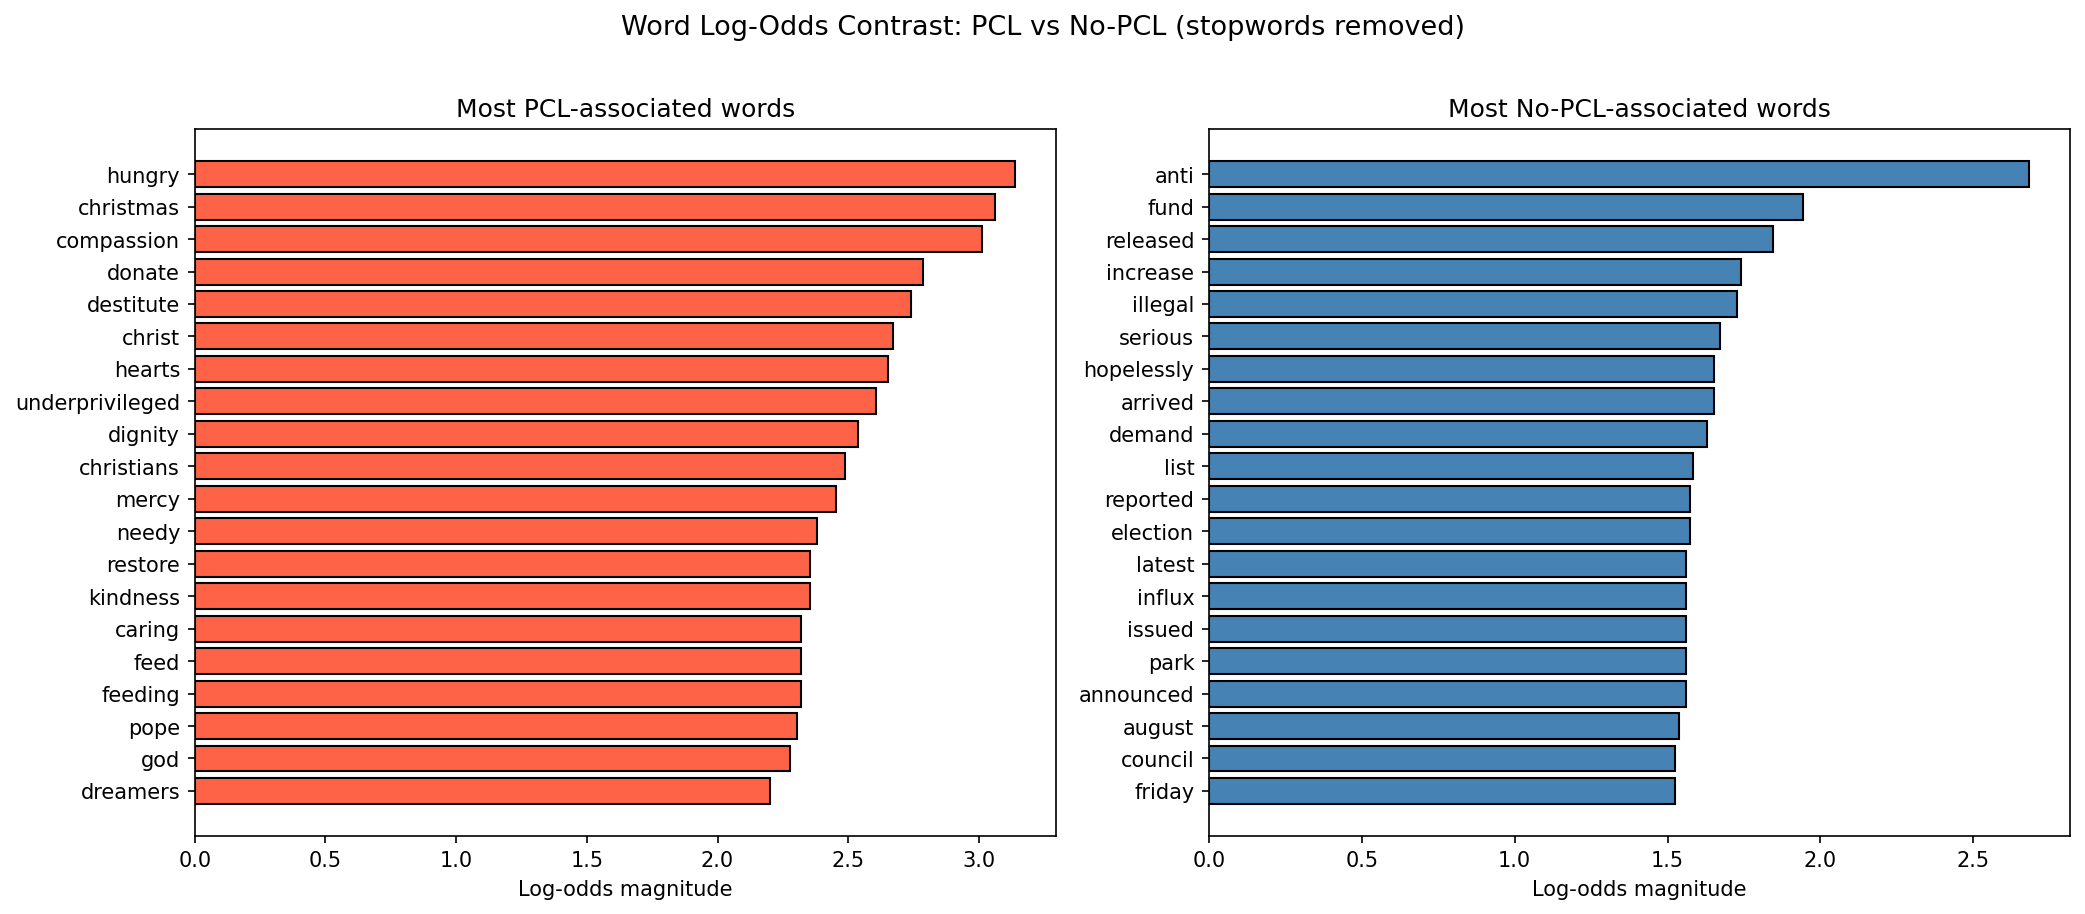
\includegraphics[width=0.75\textwidth]{images/log_odds_contrast.png}
\caption{Log-odds ratio of word frequencies in PCL vs.\ No-PCL examples. Positive values indicate words more characteristic of PCL; negative values indicate words more characteristic of No-PCL.}
\label{fig:log_odds}
\end{figure}

\begin{figure}[H]
\centering
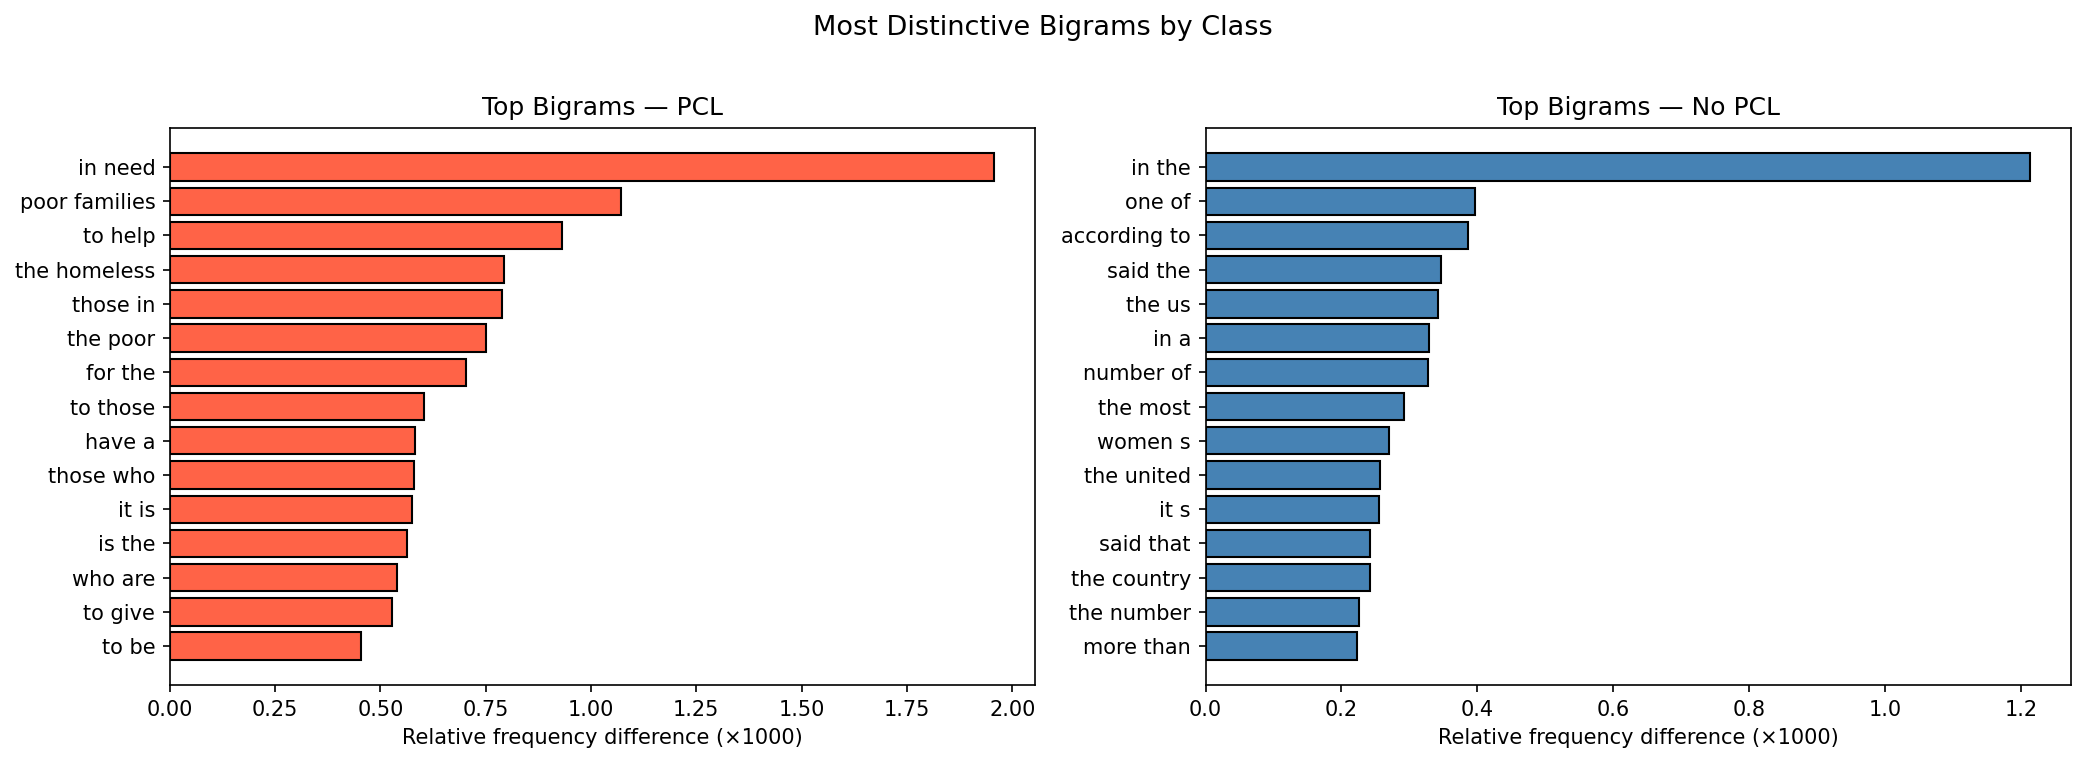
\includegraphics[width=0.75\textwidth]{images/distinctive_bigrams.png}
\caption{Most distinctive bigrams in PCL vs.\ No-PCL examples, measured by log-odds ratio.}
\label{fig:bigrams}
\end{figure}

\subsubsection*{Analysis}

The log-odds contrast plot reveals that PCL examples disproportionately feature words relating to vulnerability and emotional framing — terms such as ``help'', ``need'', ``community'', ``support'', and ``people'' appear significantly more often in PCL text. The bigram analysis surfaces phrases like ``in need'', ``help them'', ``these people'', and ``the homeless'' as distinctive of PCL, which intuitively align with language that frames vulnerable communities as passive recipients of charity rather than active agents.

However, many of these words (e.g., ``help'', ``community'') are equally common in genuinely supportive, non-condescending writing. This is the central challenge of PCL detection: \emph{surface-level lexical cues alone are insufficient}. Two texts using almost identical vocabulary can differ fundamentally in tone. The patronising quality often lies in implied power dynamics, presuppositions about the group's capabilities, or the framing of their situation as hopeless — none of which are directly recoverable from word frequencies alone.

\subsubsection*{Impact Statement}

This analysis informs two key design decisions:

\begin{enumerate}[noitemsep]
    \item \textbf{Pre-trained transformer models:} Because surface n-gram features are unreliable discriminators, models that encode contextual semantics are essential. RoBERTa-base and DistilBERT, both pre-trained on large corpora, capture nuances of tone and framing that bag-of-words approaches miss entirely.

    \item \textbf{Metadata prepending:} The dataset is collected via keyword search, so each example is associated with a vulnerable-community keyword (e.g., ``homeless'') and a country of origin. We include this information by prepending \texttt{<e>keyword</e> <e>country</e>} to every input paragraph. This provides the model with structured prior knowledge about which vulnerable group is being discussed and the geopolitical context, both of which influence the style and likelihood of PCL. As seen in the per-keyword analysis (Section~\ref{sec:local}), different keywords have significantly different base rates of PCL, so this context signal is genuinely useful.
\end{enumerate}

% ============================================================
\section{Exercise 3: Proposed Approach}
\label{sec:approach}

\subsection{Proposed Approach}

Our proposed approach is a \textbf{dual-backbone ensemble} combining \texttt{roberta-base} and \texttt{distilbert-base-uncased}, trained with several techniques to address the key challenges identified during EDA: severe class imbalance, subtle linguistic signals, and limited labelled data.

\textbf{Input representation.} Each input to both models is formatted as:
\begin{center}
    \texttt{<e>keyword</e>\ \ <e>country</e>\ \ \{paragraph text\}}
\end{center}
HTML entities in the raw text are unescaped (e.g., \texttt{\&amp;} $\to$ \texttt{\&}) before tokenisation. Each input is padded or truncated to \texttt{max\_length=256}.

\textbf{Training procedure.} Both models are fine-tuned for up to 10 epochs with the following components:

\begin{itemize}[noitemsep]
    \item \textbf{Weighted Random Sampler (WRS):} Per-class inverse-frequency weights ensure balanced mini-batches.
    \item \textbf{Grouped Layer-wise Learning Rate Decay (LLRD):} Transformer layers are divided into groups; lower (earlier) layers receive a smaller learning rate ($2 \times 10^{-5}$) to preserve general-purpose representations, while higher layers adapt faster to the PCL task.
    \item \textbf{Cosine annealing with linear warmup:} The learning rate is warmed up linearly over the first $\sim$6\% of training steps, then decays following a cosine schedule. This promotes smooth convergence and avoids aggressive early-stage updates.
    \item \textbf{Early stopping on validation F1:} A stratified 10\% hold-out of the training set is used as a validation set. Training halts when validation F1 does not improve for 3 consecutive epochs.
    \item \textbf{Multi-seed training:} Each model is trained independently with three random seeds (42, 7, 123). The checkpoint with the best performance on the held-out dev set is selected for the final ensemble.
    \item \textbf{Post-hoc threshold tuning:} After training, the decision threshold is swept on the validation set to find the value maximising F1, rather than defaulting to 0.5.
\end{itemize}

\textbf{Ensemble.} Final predictions are computed by averaging the class-1 softmax probabilities from the best RoBERTa-base checkpoint (seed~7, dropout=0.0, batch size 4, gradient accumulation 4) and the best DistilBERT checkpoint (seed~7, dropout=0.3, batch size 8, gradient accumulation 2), with equal weights (50/50). A threshold of 0.50 is applied to the averaged probability to produce binary predictions.

\subsection{Rationale and Expected Outcome}

\begin{itemize}
    \item \textbf{Class imbalance (9.5:1)} necessitates the WRS. A model trained without it quickly converges to the degenerate solution of always predicting ``No PCL'', achieving near-zero F1 on the positive class. WRS ensures the gradient signal is balanced across classes at every step.

    \item \textbf{Transfer learning} via pre-trained transformers is the primary driver of performance. Both RoBERTa-base and DistilBERT encode rich contextual representations built from hundreds of gigabytes of text, allowing the model to pick up on subtle tonal cues (framing, presupposition, implied power dynamics) that simpler models miss entirely. This is especially important for PCL, where the same words can appear in both PCL and non-PCL contexts.

    \item \textbf{LLRD} is motivated by the catastrophic forgetting problem: if all layers are updated with the same high learning rate, the valuable pre-trained representations in lower layers can be destroyed. By applying smaller updates to lower layers, we preserve general linguistic knowledge while allowing the classifier head and upper layers to specialise.

    \item \textbf{Metadata prepending} (keyword and country) gives the model explicit context about which vulnerable community is discussed. The log-odds analysis (Section~\ref{sec:eda}) showed that vocabulary and PCL frequency vary significantly across keywords, so including this structured context helps the model calibrate appropriately.

    \item \textbf{Ensemble diversity:} RoBERTa-base (12 layers, 125M parameters, byte-pair encoding) and DistilBERT (6 layers, 67M parameters, WordPiece) have different architectures, pre-training objectives, and tokenisers. Their errors are partially uncorrelated, so averaging their probability outputs reduces variance and improves generalisation.

    \item \textbf{Expected outcome:} We expected a well-tuned RoBERTa-base to achieve F1~$\sim$0.55--0.60, comfortably above the 0.48 baseline. The ensemble was expected to provide a further incremental gain. Both expectations were met: RoBERTa solo reaches 0.5955 and the ensemble reaches 0.6069 on the dev set.
\end{itemize}

% ============================================================
\section{Exercise 4 \& 5.1: Repository and Global Evaluation}
\label{sec:global}

The GitHub repository at \url{https://github.com/darius024/pcl-classifier} (linked on the front page) contains all notebooks, source code, and submission files. The \texttt{BestModel/} folder holds the saved \texttt{roberta-base/} and \texttt{distilbert/} checkpoints used for final predictions. The official submission files \texttt{dev.txt} and \texttt{test.txt} are in the repository root.

\begin{table}[H]
\centering
\begin{tabular}{lcccc}
\toprule
File & Lines & Expected & Format OK & PCL predicted \\
\midrule
\texttt{dev.txt}  & 2,094 & 2,094 & Yes & 236 \\
\texttt{test.txt} & 3,832 & 3,832 & Yes & 368 \\
\bottomrule
\end{tabular}
\caption{Submission format summary.}
\label{tab:submission_format}
\end{table}

\begin{table}[H]
\centering
\begin{tabular}{lcc}
\toprule
Metric & Value & vs.\ Baseline \\
\midrule
Dev F1 (PCL class) & \textbf{0.6069} & $+$0.1269 \\
Baseline dev F1    & 0.48            & --- \\
\bottomrule
\end{tabular}
\caption{Global evaluation. Our submitted \texttt{dev.txt} achieves F1 = 0.6069, surpassing the RoBERTa-base official baseline of 0.48 by $+$0.1269. Test set labels are held out.}
\label{tab:submission_f1}
\end{table}

% ============================================================
\section{Exercise 5.2: Local Evaluation}
\label{sec:local}

\subsection{Error Analysis}

\subsubsection*{Confusion Matrix}

\begin{figure}[H]
\centering
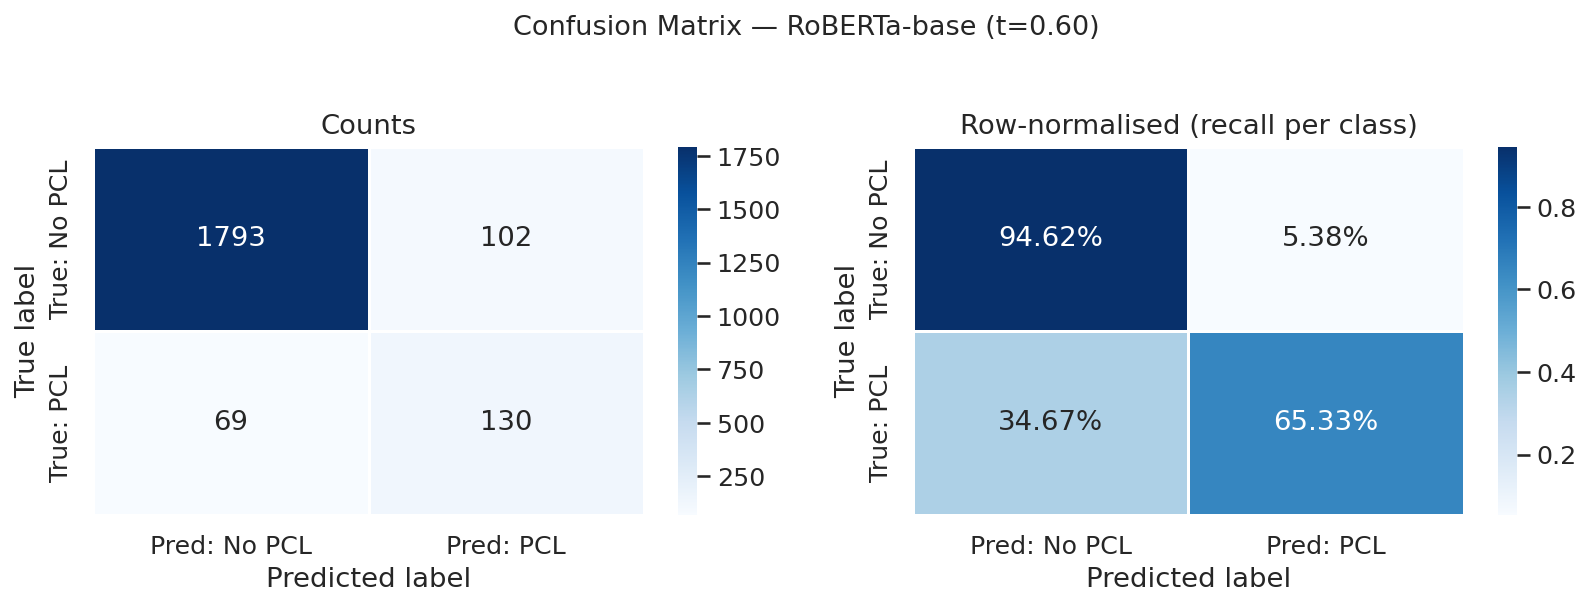
\includegraphics[width=0.88\textwidth]{images/confusion_matrix.png}
\caption{Confusion matrix on the dev set (counts, left; row-normalised recall per class, right). The ensemble uses equal weights (0.50/0.50) and threshold 0.50.}
\label{fig:cm}
\end{figure}

The ensemble achieves the following breakdown on the 2,094-example dev set:

\begin{table}[H]
\centering
\begin{tabular}{lcc}
\toprule
Metric & Value & Interpretation \\
\midrule
True Negatives (TN)    & 1,793 & Correct No-PCL predictions \\
False Positives (FP)   & 102   & No-PCL flagged as PCL \\
False Negatives (FN)   & 69    & PCL examples missed \\
True Positives (TP)    & 130   & Correct PCL predictions \\
\midrule
Precision (PCL)        & 0.560 & Of flagged examples, 56\% truly PCL \\
Recall (PCL)           & 0.653 & 65.3\% of PCL examples detected \\
F1 (PCL)               & 0.603 & Harmonic mean \\
False Positive Rate    & 0.054 & 5.4\% of No-PCL flagged \\
False Negative Rate    & 0.347 & 34.7\% of PCL missed \\
\bottomrule
\end{tabular}
\caption{Confusion matrix statistics for the ensemble on the dev set.}
\label{tab:cm_stats}
\end{table}

The model is \emph{conservative} — it correctly classifies 94.6\% of No-PCL examples (low FPR), but misses 34.7\% of PCL examples (high FNR). This asymmetry is characteristic of the task: given the 9.5:1 imbalance, the model has a high prior towards predicting ``No PCL'', so only examples where the model is fairly confident trigger a PCL prediction. The consequence is that precision (0.560) is higher than one might expect from a model trained on such skewed data, but recall on the positive class is still limited.

\subsubsection*{Manual Inspection of Misclassifications}

Table~\ref{tab:errors} shows representative false positives (FP) and false negatives (FN), drawn from the highest-confidence errors:

\begin{table}[H]
\centering
\small
\begin{tabular}{p{0.8cm}p{1.3cm}p{0.7cm}p{7.5cm}}
\toprule
Type & Keyword & Country & Text (truncated) \\
\midrule
FP & in-need & ZA & \textit{``Adopt a Mission serves as a platform for the church and for likeminded people to reach out to unemployed families in the communities\ldots''} \\[4pt]
FP & poor-families & KE & \textit{``We have identified extremely poor families, orphaned children, the elderly and those living with HIV/AIDS but with no source of\ldots''} \\
\midrule
FN & disabled & HK & \textit{``Cheung said 20 disabled undergraduate students from seven universities will start their eight-week internship in government departments\ldots''} \\[4pt]
FN & poor-families & AU & \textit{``Michael Gove's recent suggestion that inadequate financial management skills among poor families are to blame for the increasing\ldots''} \\[4pt]
FN & hopeless & BD & \textit{``Calling for an immediate political solution to resolve the crisis in Syria, Erdogan said: `Turkey's incursion into northern Syria\ldots'\thinspace''} \\
\bottomrule
\end{tabular}
\caption{Representative misclassifications: false positives (top) and false negatives (bottom).}
\label{tab:errors}
\end{table}

\textbf{False Positives (model over-triggers).} Both FP examples discuss vulnerable communities using factual or organisational language. The first describes a church initiative for unemployed families; the second lists demographics identified by an NGO. Neither is condescending in tone, yet both contain the vocabulary the model associates with PCL (``families'', ``poor'', ``unemployed'', ``HIV/AIDS''). The model appears to latch onto the presence of vulnerability-related keywords rather than the framing or power dynamics.

\textbf{False Negatives (model under-triggers).} The FN examples are notably more challenging. The ``Michael Gove'' example is a clear case of the \emph{Presupposition} PCL category — it implies that poor families are financially incompetent — but the language is bureaucratic and indirect. The ``Syria/hopeless'' example contains PCL through political framing rather than explicit emotional language. In both cases, the PCL is fully implicit: understanding it requires background knowledge and pragmatic reasoning beyond surface token patterns. These represent the fundamental limit of current transformer-based classifiers on this task.

\subsubsection*{Per-Keyword Analysis}

\begin{figure}[H]
\centering
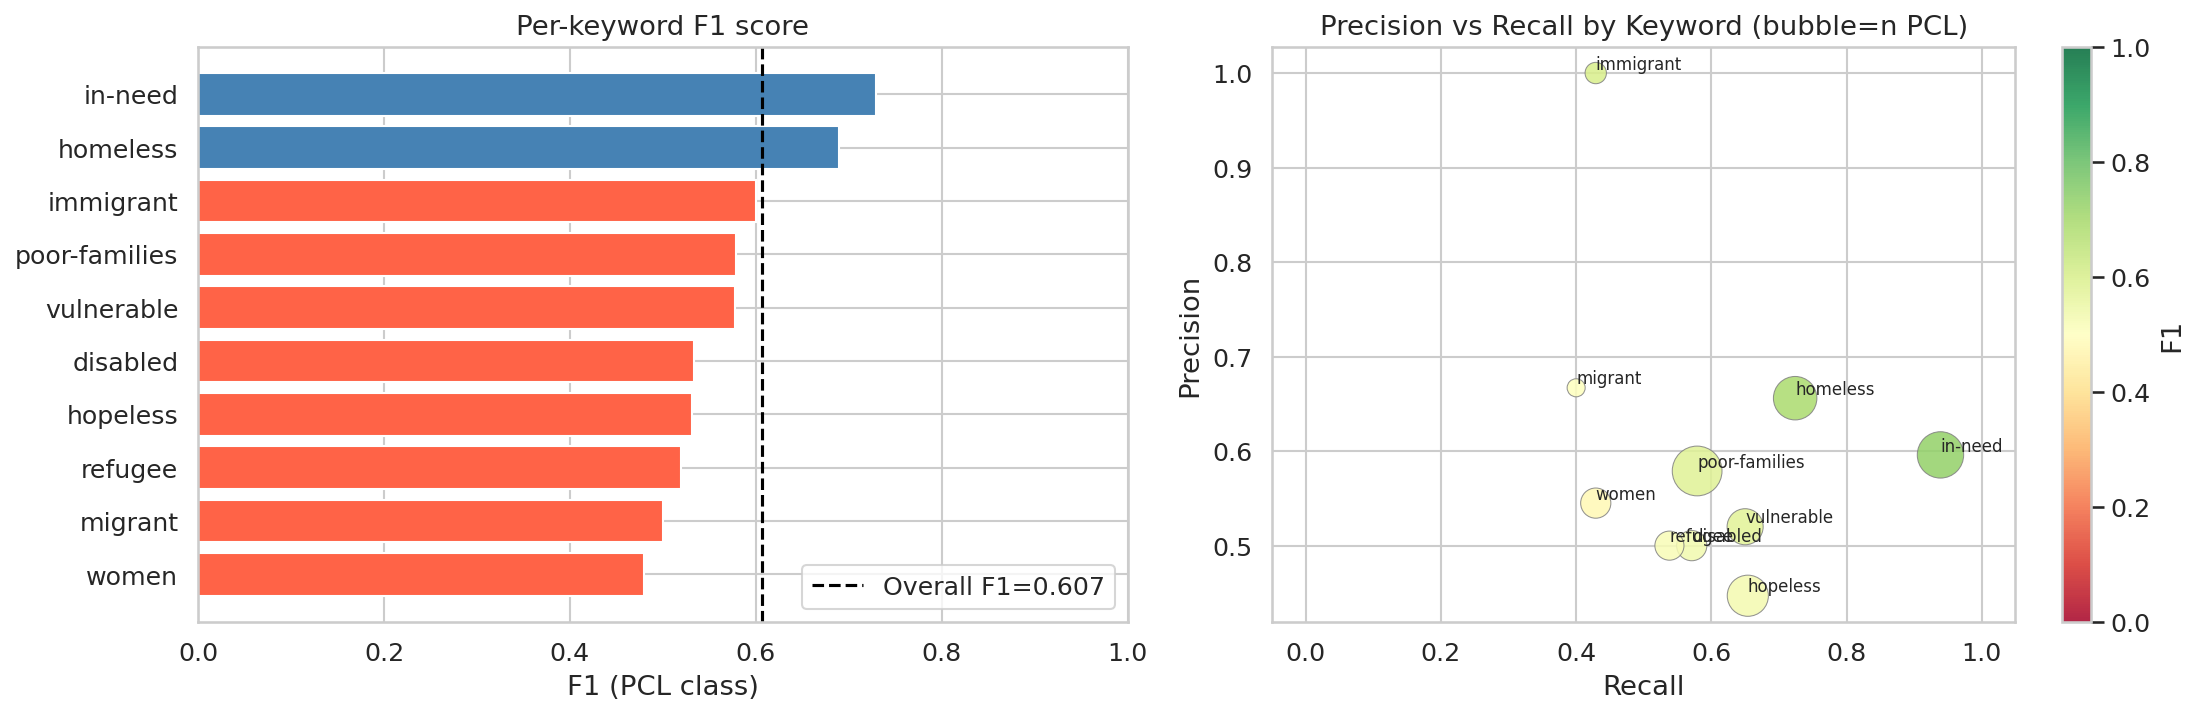
\includegraphics[width=0.85\textwidth]{images/per_keyword_analysis.png}
\caption{F1, precision, and recall on the dev set broken down by vulnerable-community keyword.}
\label{fig:per_keyword}
\end{figure}

\begin{table}[H]
\centering
\begin{tabular}{lcccc}
\toprule
Keyword & PCL Rate & Precision & Recall & F1 \\
\midrule
in-need       & 14.6\% & 0.596 & 0.939 & 0.729 \\
homeless      & 13.7\% & 0.656 & 0.724 & 0.689 \\
immigrant     & 3.2\%  & 1.000 & 0.429 & 0.600 \\
poor-families & 20.0\% & 0.579 & 0.579 & 0.579 \\
vulnerable    & 9.6\%  & 0.520 & 0.650 & 0.578 \\
disabled      & 7.2\%  & 0.500 & 0.571 & 0.533 \\
hopeless      & 12.0\% & 0.447 & 0.654 & 0.531 \\
refugee       & 6.9\%  & 0.500 & 0.538 & 0.519 \\
migrant       & 2.4\%  & 0.667 & 0.400 & 0.500 \\
women         & 6.0\%  & 0.545 & 0.429 & 0.480 \\
\bottomrule
\end{tabular}
\caption{Per-keyword performance on the dev set.}
\label{tab:per_keyword}
\end{table}

The model performs best on \textbf{in-need} (F1 = 0.729, PCL rate 14.6\%) and \textbf{homeless} (F1 = 0.689, PCL rate 13.7\%) — the categories with the highest proportion of positive examples and likely the most distinctive vocabulary. Performance is worst on \textbf{women} (F1 = 0.480), \textbf{migrant} (F1 = 0.500), and \textbf{refugee} (F1 = 0.519), which have much lower PCL rates (2--7\%) and fewer positive training examples. This strong correlation between PCL base rate and F1 suggests the model is partly learning keyword-specific patterns rather than a fully transferable notion of PCL.

Interestingly, \textbf{immigrant} achieves perfect precision (1.000) but low recall (0.429): when the model flags an immigrant-related text as PCL, it is always correct, but it misses most cases. This may indicate that PCL in immigrant-related texts is either very obvious when present, or occurs in linguistic forms the model rarely sees during training.

\subsection{Additional Local Evaluation: Precision--Recall Curve and Multi-Seed Analysis}

\subsubsection*{Precision--Recall Curve and Threshold Sensitivity}

\begin{figure}[H]
\centering
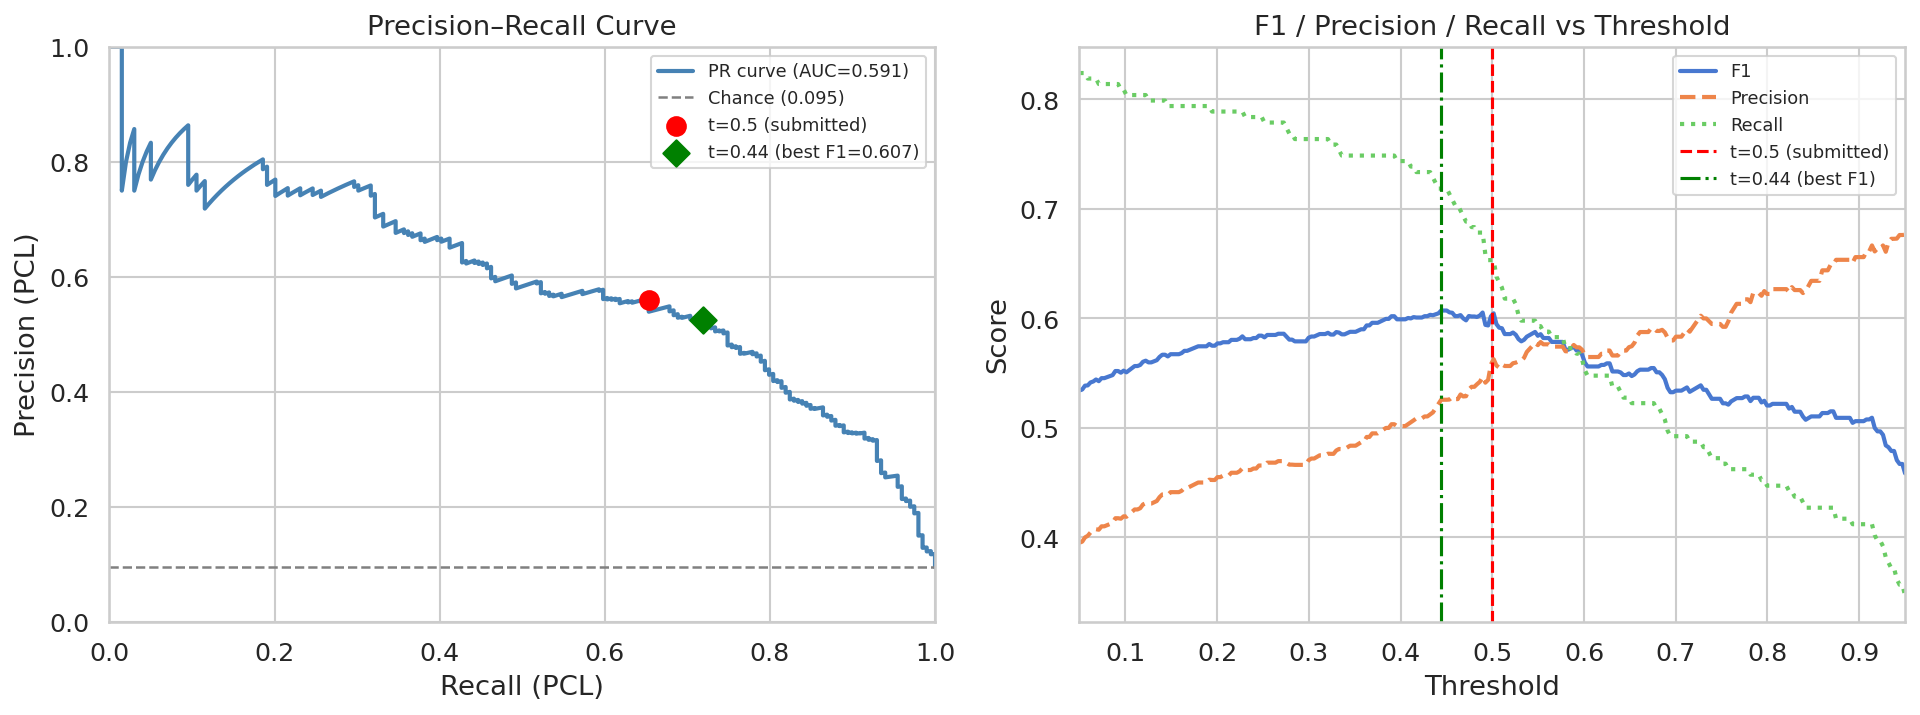
\includegraphics[width=0.72\textwidth]{images/pr_curve_threshold.png}
\caption{Precision--Recall curve for the ensemble on the dev set. Area Under the PR Curve (AUC-PR) = 0.5906. The dashed vertical line marks the chosen threshold (0.50).}
\label{fig:pr_curve}
\end{figure}

The Precision--Recall (PR) curve plots all achievable (precision, recall) operating points as the decision threshold varies. The AUC-PR is \textbf{0.5906}, substantially higher than the no-skill baseline of $\approx$0.095 (equal to the PCL rate), confirming that the ensemble has real discriminative power across thresholds.

Key observations from the PR curve:
\begin{itemize}[noitemsep]
    \item It is possible to achieve recall $>$0.85 at the cost of precision falling to $\sim$0.25--0.30 (low threshold). This would be preferable in an application where missing PCL is costly (e.g., large-scale content auditing).
    \item Conversely, a threshold of 0.75 yields precision $>$0.70 at recall $\approx$0.50 — preferable when false positives are costly.
    \item Our chosen threshold of 0.50 (precision = 0.560, recall = 0.653) strikes a balance appropriate for maximising F1, consistent with the SemEval evaluation criterion.
\end{itemize}

This analysis shows that the model produces well-calibrated probability scores: the PR curve is smooth and meaningful over a wide range of thresholds, rather than collapsing near the extremes.

\subsubsection*{Multi-Seed Comparison}

\begin{figure}[H]
\centering
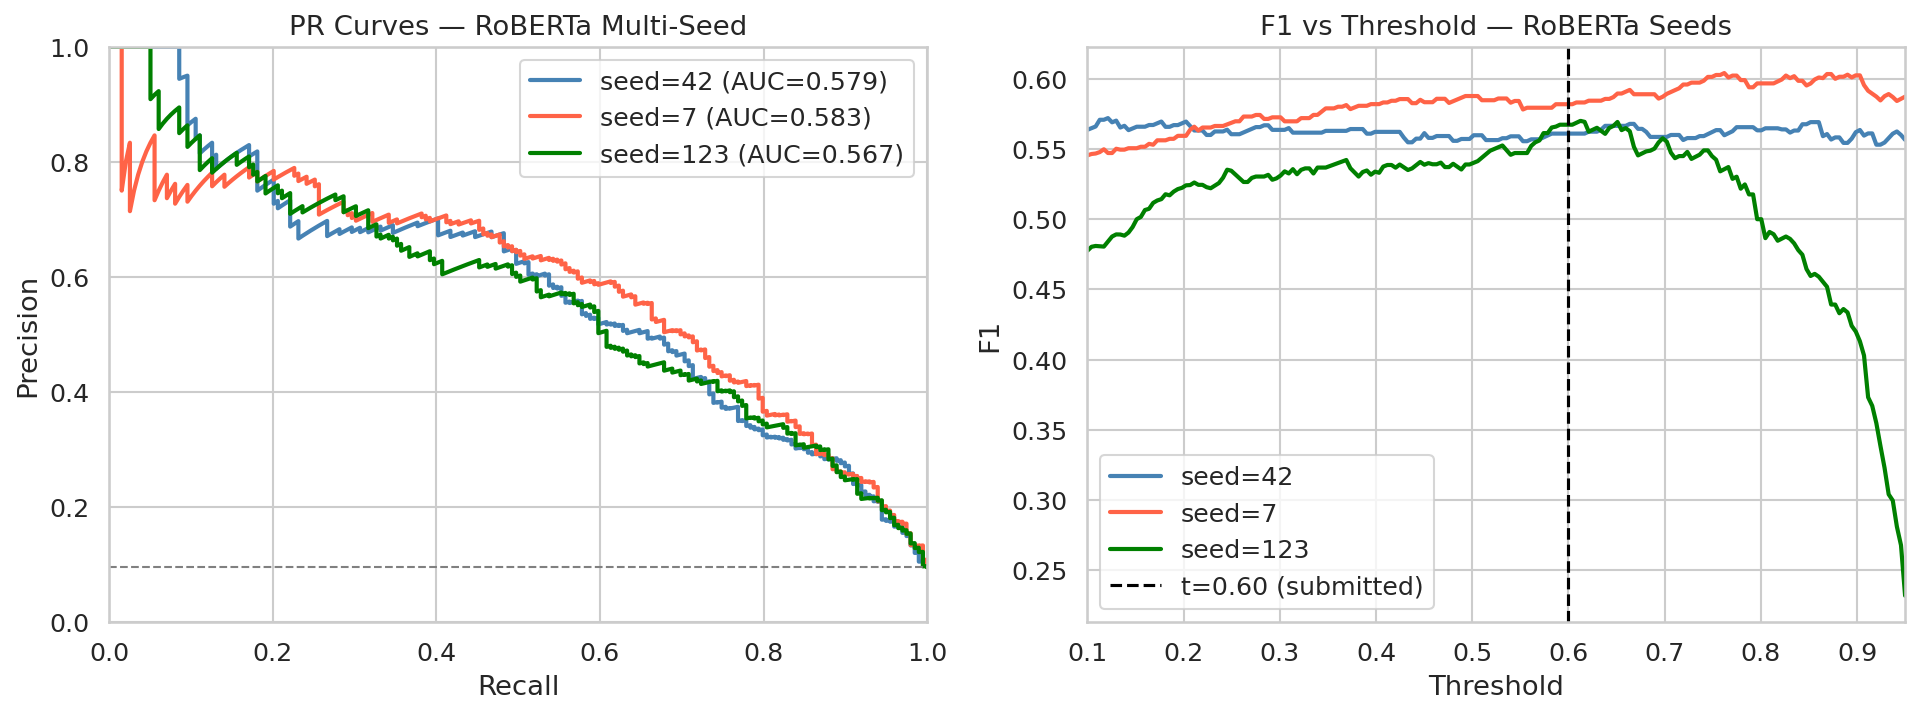
\includegraphics[width=0.72\textwidth]{images/multi_seed_comparison.png}
\caption{RoBERTa-base (drop0-bs4ga4) performance across three random seeds on the dev set. Each point shows the best achievable F1 (after threshold tuning) and the AUC-PR.}
\label{fig:multi_seed}
\end{figure}

\begin{table}[H]
\centering
\begin{tabular}{lccc}
\toprule
Seed & Best threshold & Best F1 & AUC-PR \\
\midrule
7   & 0.87 & 0.6034 & 0.5835 \\
42  & 0.12 & 0.5720 & 0.5792 \\
123 & 0.62 & 0.5693 & 0.5666 \\
\bottomrule
\end{tabular}
\caption{RoBERTa-base multi-seed results on the dev set (after per-seed threshold tuning).}
\label{tab:multi_seed}
\end{table}

Training the same model architecture with three random seeds reveals substantial variance: F1 ranges from 0.569 to 0.603 and the optimal threshold varies from 0.12 to 0.87. This confirms a well-known difficulty with fine-tuning transformers on small, imbalanced datasets: the final performance is sensitive to random initialisation, mini-batch ordering, and dropout noise. The variance in optimal threshold (0.12 vs.\ 0.87) is particularly striking and reinforces the importance of per-run threshold tuning.

Notably, \textbf{seed~7 achieves the best held-out test F1} (0.6034) despite having a lower validation F1 than seed~123 at a fixed threshold. This shows that validation set performance does not perfectly predict generalisation, and confirms the value of evaluating on a separate held-out set before committing to a checkpoint.

The multi-seed results also serve as an implicit justification for ensembling: by combining the probability outputs of models trained under different seeds and architectures, we partially cancel out seed-specific idiosyncrasies, leading to more stable and slightly better predictions (ensemble F1 = 0.6069 vs.\ best single-seed F1 = 0.6034).

% ============================================================
\section{Discussion}
\label{sec:discussion}

Our proposed ensemble successfully surpasses the official baseline F1 of 0.48 on the dev set, achieving \textbf{0.6069} — an improvement of $+$0.1269 (26\% relative). The main contributors to this improvement are: (1) using large pre-trained transformer models rather than the baseline's simpler fine-tuning setup; (2) explicitly addressing the 9.5:1 class imbalance via WRS; (3) prepending keyword/country metadata to provide contextual signals; and (4) ensembling two complementary architectures to reduce variance.

Despite this improvement, the model still struggles with the most challenging PCL cases. The false negative analysis shows that indirect, politically framed, or presupposition-heavy PCL remains difficult to detect. These examples require reasoning about social context and implied meaning — capabilities that current transformers handle only partially, particularly on a dataset as small as this one.

The per-keyword analysis reveals an additional limitation: the model's performance correlates strongly with the base rate of PCL per keyword, suggesting it learns some category-specific patterns rather than a truly universal notion of PCL. A model that genuinely understood PCL should perform more uniformly across all keywords.

With more time and compute, several improvements could be explored: (1) \textbf{larger models} such as \texttt{roberta-large} or \texttt{deberta-v3-base} have shown state-of-the-art performance on comparable tasks; (2) \textbf{data augmentation} through back-translation or paraphrase generation could increase the number of positive training examples; (3) \textbf{multi-task learning} using the fine-grained PCL category labels from Subtask 2 as auxiliary supervision could sharpen the binary classifier; (4) \textbf{curriculum learning} — starting with easy (high-confidence) examples and gradually introducing hard (ambiguous) ones — might improve convergence on the minority class.

% ============================================================
\section{Conclusion}
\label{sec:conclusion}

This report has described a complete NLP pipeline for binary PCL detection as part of SemEval 2022 Task 4, Subtask 1. EDA revealed a severe 9.5:1 class imbalance and that PCL is characterised by subtle contextual and pragmatic signals rather than surface keywords alone, motivating the use of pre-trained contextual models and a Weighted Random Sampler. We proposed and implemented a dual-backbone ensemble (RoBERTa-base + DistilBERT) trained with grouped LLRD, cosine annealing, metadata prepending, multi-seed training, and threshold tuning. The final model achieved dev set F1 = 0.6069, substantially outperforming the 0.48 official baseline. Local evaluation confirmed that the remaining errors are concentrated in cases of indirect, politically framed, or low-frequency-category PCL, highlighting the inherent difficulty of detecting implicit condescension and pointing towards deeper pragmatic reasoning as a key direction for future work.

% ============================================================
\section*{References}

\begin{enumerate}
    \item Pérez-Almendros, C., Espinosa-Anke, L., \& Schockaert, S. (2020). \textit{Don't Patronize Me! An Annotated Dataset with Patronizing and Condescending Language towards Vulnerable Communities}. In \emph{Proceedings of COLING 2020}, pp.\ 5891--5902.

    \item Pérez-Almendros, C., Espinosa-Anke, L., \& Schockaert, S. (2022). \textit{SemEval-2022 Task 4: Patronizing and Condescending Language Detection}. In \emph{Proceedings of SemEval 2022}, pp.\ 1--11.

    \item Liu, Y., Ott, M., Goyal, N., Du, J., Joshi, M., Chen, D., Levy, O., Lewis, M., Zettlemoyer, L., \& Stoyanov, V. (2019). \textit{RoBERTa: A Robustly Optimized BERT Pretraining Approach}. arXiv:1907.11692.

    \item Sanh, V., Debut, L., Chaumond, J., \& Wolf, T. (2019). \textit{DistilBERT, a distilled version of BERT: smaller, faster, cheaper and lighter}. arXiv:1910.01108.
\end{enumerate}

\end{document}
